%========================abstract=========================
\section*{Executive Summary}
\begin{comment}
%\addcontentsline{toc}{section}{Abstract}
%\noindent Agricultural intensification, mechanization, and automation have all led to major increases in agricultural productivity throughout time \cite{nof2009springer}. Robots are intelligent machines that may be trained to carry out particular jobs, make choices, and take immediate action. They are needed in a variety of industries where less labor is often needed, and they function best in stable environments where consistent accuracy and high productivity are required \cite{nof1999handbook}.\\
%~\\
%\noindent LEF BOTS GmbH is a robot specialising company, the name of the firm is created from the initials of the stakeholders: \textbf{L}aura; \textbf{E}ncarnacion; \textbf{F}erlando \textbf{(LEF)}. In this text, the firm presents the development of its major product; the fruit harvesting robot. The robot is given an intuitive name \textbf{Fruta Oes}, which is a combination of two languages Spanish and Afrikaans. Fruta means fruits in Spanish and Oes means to harvest in Afrikaans, thus, the name of the robot \textbf{Fruta Oes} means fruits harvester. One might be asking themselves why Spanish and Afrikaans, well the answer is simple, the stakeholders of the firm are from Spain (Laura and Encarnacion) and South Africa (Ferlando). \Vref{fig:2oppositeviews} Presents \textbf{Fruta Oes}.
\end{comment}

\noindent This document illustrates the process to develop a robot using the Scrum methodology. It was part of the Computer Science lecture and was designed to introduce students to Scrum and software development.
The Scrum methodology will be used to manage the project, which involves dividing the project into small, manageable parts called sprints. Each sprint will have specific goals and will last for a week.

\begin{figure}[h]
	\centering
	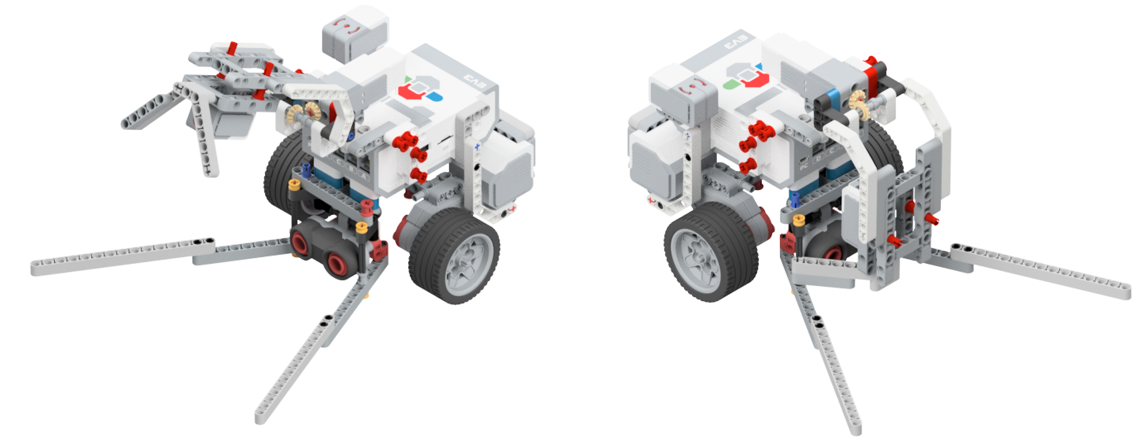
\includegraphics[width=\linewidth]{Graphics/2oppositeViews}
	\caption{Fruta Oes}
	\label{fig:2oppositeviews}
\end{figure}

\begin{comment}
	\noindent The robot mechanical structure is the most important part of this project therefore, this document will discuss in detail all the sub-components of the mechanical design in \vref{sec:mechanicalDesign}. Following by the software design where a full discussion on all the algorithms used, activity diagrams and testing will be provided in \vref{sec:softwareDesign}. Following will be the management of the software development, \vref{sec:softwareEngineering} highlights the Agile Software engineering (SCRUM) procedure followed in this project. The SCRUM section will briefly discuss the project setup in \vref{sec:projectSetup}, then \cref{sec:sprint1}, \cref{sec:sprint2},\cref{sec:sprint3} present the role and progress achieved in sprint 1, sprint 2 and sprint 3 respectively. Finally, recommendations will be detailed in \vref{sec:RecommendationsAndConclusion} then in the same section this document will go into a concluding discussion....
\end{comment}

\noindent The team will begin by defining the requirements of the robot and creating a product backlog. The team will then hold a sprint planning meeting to determine which tasks will be completed during the next sprint. During each sprint, the development team will work on building the robot, and the Scrum Master will hold daily stand-up meetings to ensure that everyone is on track and that any obstacles are addressed. The team will also hold a sprint review meeting at the end of each sprint to review what has been accomplished and plan for the next sprint.
Once the robot is completed, it will be tested to ensure that it meets the requirements and that it is able to perform the task for which it was designed. The team will hold a retrospective meeting to review the project and identify any areas for improvement for future projects.
By using the Scrum methodology, the project will be well-organized and efficient, and the final product will be a high-quality, functional robot that is capable of performing its main task: harvesting fruits.

This task makes the robot’s mechanical structure the most important part. Thus, this document will discuss in detail all the sub-components of the mechanical design in \vref{sec:mechanicalDesign}, followed in \vref{sec:softwareDesign} by the software design where a full discussion on all the algorithms used, activity diagrams and testing will be provided. The next step will be the management of the software development: \vref{sec:softwareEngineering} highlights the Agile Software engineering (SCRUM) procedure followed in this project. The SCRUM section will briefly discuss the project setup in \vref{sec:projectSetup}. Then \cref{sec:sprint1}, \cref{sec:sprint2},\cref{sec:sprint3} present the role and progress achieved in sprints 1, 2, and 3 respectively. Finally, discussions and reflections will be detailed in \vref{sec:RecommendationsAndConclusion} 







